\documentclass[border=4pt]{standalone}
\usepackage{fontspec}
\setmainfont{DMSans9pt}[Path=../../fonts/, Extension=.ttf, UprightFont=*-Regular, BoldFont=*-Bold, ItalicFont=*-Italic, BoldItalicFont=*-BoldItalic]
\setsansfont{DMSans9pt}[Path=../../fonts/, Extension=.ttf, UprightFont=*-Regular, BoldFont=*-Bold, ItalicFont=*-Italic, BoldItalicFont=*-BoldItalic]
\usepackage{amsmath,amssymb,xcolor}
\usepackage{tikz}
\usetikzlibrary{arrows.meta,positioning,shapes.geometric,shapes.misc,fit,backgrounds,calc,decorations.pathreplacing,shadows}
\definecolor{cTwo}{HTML}{4C72B0}
\definecolor{cOne}{HTML}{DD8452}
\definecolor{cDetr}{HTML}{55A868}
\definecolor{cOvd}{HTML}{8172B3}
\definecolor{cAgent}{HTML}{C44E52}
\definecolor{cEdge}{HTML}{937860}
\definecolor{cApp}{HTML}{DA8BC3}
\definecolor{cData}{HTML}{4C9BB0}

\makeatletter
\def\refmap#1#2{\expandafter\def\csname rm@#1\endcsname{#2}}
\def\rm@ref#1{\csname rm@#1\endcsname}
\renewcommand{\ref}{\@ifstar\rm@ref\rm@ref}
\renewcommand{\eqref}[1]{(\csname rm@#1\endcsname)}
\makeatother

\refmap{eq:ciou}{10}\refmap{eq:detector}{1}\refmap{eq:dfl}{11}\refmap{eq:giou}{9}\refmap{eq:glip}{17}\refmap{eq:grpo}{20}\refmap{eq:infonce}{15}\refmap{eq:mllm-box}{19}\refmap{eq:ovd}{2}\refmap{eq:reparam}{18}\refmap{eq:roialign}{6}\refmap{eq:rpn}{5}\refmap{eq:siglip}{16}\refmap{eq:tal}{8}\refmap{sec:agentic}{5}\refmap{sec:closed}{3}\refmap{sec:manufacturing}{7.1}\refmap{sec:mllm-direct}{5.1}\refmap{sec:mllm-rl}{5.2}\refmap{sec:mllm-tools}{5.3}\refmap{sec:ovd}{4}\refmap{sec:ovd-distill}{4.2}\refmap{sec:ovd-grounding}{4.3}\refmap{sec:ovd-owl}{4.4}\refmap{sec:ovd-rt}{4.5}\refmap{sec:ovd-unified}{4.6}\refmap{sec:twostage}{3.1}\refmap{sec:vlfound}{4.1}\refmap{sec:yolo}{3.3}\refmap{tab:yolo}{4}
%% ---------- illustrative scene thumbnails (drawn, not photographs); origin = lower-left, size 2.4 x 1.7
\definecolor{pcbG}{HTML}{2E7D4F}\definecolor{pcbD}{HTML}{1F5A39}\definecolor{chipK}{HTML}{2B2B2B}
\definecolor{soil}{HTML}{8B6B4A}\definecolor{soilD}{HTML}{6E5238}\definecolor{crop}{HTML}{6BB04A}\definecolor{weed}{HTML}{3E7C2A}
\definecolor{belt}{HTML}{5A5F66}\definecolor{carton}{HTML}{C9A46A}\definecolor{cartonD}{HTML}{A9844C}\definecolor{pallet}{HTML}{9C7A4F}
\tikzset{bx/.style={draw=#1, line width=0.8pt}, bxl/.style={fill=#1, text=white, font=\fontsize{4.2}{4.2}\selectfont\bfseries, inner sep=0.6pt, anchor=south west}}
% PCB: chips, pads, one solder bridge
\newcommand{\scenePCB}{%
  \fill[pcbG, rounded corners=1pt] (0,0) rectangle (2.4,1.7);
  \foreach \y in {0.25,0.55,0.85,1.15,1.45}{\draw[pcbD, line width=0.35pt] (0.05,\y) -- (2.35,\y);}
  \fill[chipK] (0.25,0.75) rectangle (0.95,1.4);
  \foreach \x in {0.32,0.47,0.62,0.77,0.89}{\fill[gray!60] (\x-0.03,0.66) rectangle (\x+0.03,0.75); \fill[gray!60] (\x-0.03,1.4) rectangle (\x+0.03,1.49);}
  \fill[chipK] (1.35,0.2) rectangle (2.15,0.7);
  \foreach \x in {1.45,1.65,1.85,2.05}{\fill[gray!60] (\x-0.04,0.7) rectangle (\x+0.04,0.8);}
  \fill[gray!70] (1.7,1.05) circle (0.07); \fill[gray!70] (1.95,1.05) circle (0.07); \fill[gray!70] (2.2,1.05) circle (0.07);
  \fill[gray!75] (1.7,1.0) rectangle (1.95,1.1); % bridge between pads
}
% Field: soil rows with crops and weeds
\newcommand{\sceneField}{%
  \fill[soil, rounded corners=1pt] (0,0) rectangle (2.4,1.7);
  \foreach \y in {0.35,0.85,1.35}{\fill[soilD] (0.05,\y-0.06) rectangle (2.35,\y+0.06);}
  \foreach \x/\y in {0.3/0.35,0.8/0.35,1.3/0.35,1.8/0.35,0.3/0.85,0.8/0.85,1.8/0.85,2.2/0.85,0.55/1.35,1.05/1.35,1.55/1.35,2.05/1.35}{%
    \fill[crop] (\x,\y) ellipse (0.11 and 0.07); \fill[crop] (\x,\y+0.05) ellipse (0.05 and 0.1);}
  \foreach \x/\y in {1.3/0.85,0.6/0.6}{\foreach \a in {0,60,...,300}{\fill[weed, rotate around={\a:(\x,\y)}] (\x+0.07,\y) ellipse (0.07 and 0.025);}}
}
% Warehouse: belt with cartons and a pallet stack
\newcommand{\sceneWarehouse}{%
  \fill[gray!15, rounded corners=1pt] (0,0) rectangle (2.4,1.7);
  \fill[belt] (0,0.15) rectangle (2.4,0.45);
  \foreach \x in {0.1,0.5,...,2.3}{\draw[gray!50, line width=0.3pt] (\x,0.15) -- (\x,0.45);}
  \fill[carton] (0.2,0.45) rectangle (0.75,0.85); \draw[cartonD] (0.475,0.45) -- (0.475,0.85);
  \fill[carton] (1.0,0.45) rectangle (1.4,0.75); \draw[cartonD] (1.2,0.45) -- (1.2,0.75);
  \fill[pallet] (1.6,0.55) rectangle (2.3,0.65);
  \fill[carton] (1.62,0.65) rectangle (1.95,0.95); \fill[carton] (1.97,0.65) rectangle (2.28,0.95); \fill[carton] (1.75,0.95) rectangle (2.15,1.25);
  \draw[cartonD] (1.62,0.65) rectangle (1.95,0.95); \draw[cartonD] (1.97,0.65) rectangle (2.28,0.95); \draw[cartonD] (1.75,0.95) rectangle (2.15,1.25);
}
% Metal surface with scratch and dent
\newcommand{\sceneSurface}{%
  \shade[left color=gray!35, right color=gray!15, rounded corners=1pt] (0,0) rectangle (2.4,1.7);
  \foreach \i in {1,...,14}{\draw[gray!45, line width=0.2pt] (0.05,0.1*\i) -- (2.35,0.1*\i+0.03);}
  \draw[gray!80!black, line width=0.6pt] (0.4,1.25) .. controls (0.8,1.15) and (1.0,1.05) .. (1.35,0.95);
  \fill[gray!65] (1.8,0.45) ellipse (0.16 and 0.1);
}

\begin{document}
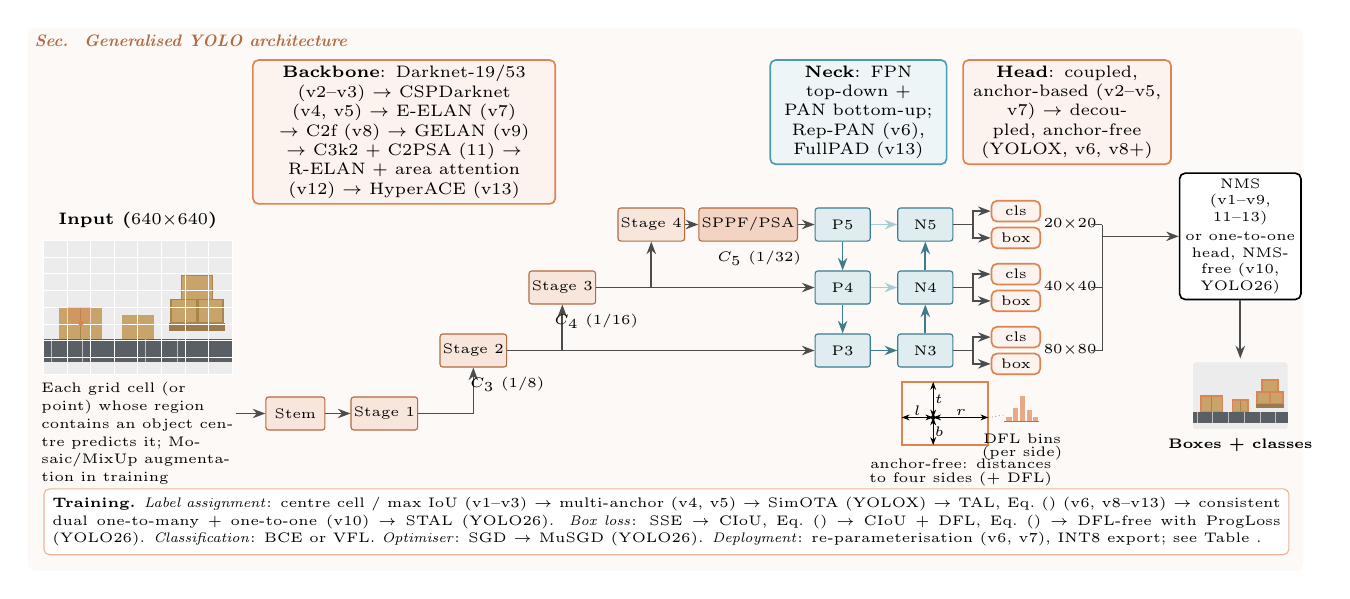
\begin{tikzpicture}[
  font=\fontsize{6}{7}\selectfont,
  mod/.style={draw=#1, fill=#1!10, rounded corners=2pt, line width=0.6pt, align=center, inner sep=2pt},
  tag/.style={fill=#1, text=white, rounded corners=1.5pt, font=\fontsize{5}{5.8}\selectfont\bfseries, inner sep=1.3pt, align=center},
  sec/.style={font=\fontsize{6.2}{7}\selectfont\bfseries\itshape, text=#1, anchor=north west, inner sep=1pt},
  arr/.style={-{Stealth[length=1.6mm]}, line width=0.6pt, black!70},
  note/.style={font=\fontsize{5.4}{6.4}\selectfont, align=justify, text width=#1, inner sep=0pt},
  stg/.style={draw=cOne!80!black, fill=cOne!20, rounded corners=1pt, minimum width=0.75cm, minimum height=0.42cm, font=\fontsize{5}{5}\selectfont, inner sep=1pt},
  nk/.style={draw=cData!80!black, fill=cData!18, rounded corners=1pt, minimum width=0.7cm, minimum height=0.42cm, font=\fontsize{5}{5}\selectfont, inner sep=1pt},
]
\fill[cOne!5, rounded corners=3pt] (-0.2,-0.95) rectangle (16.0,5.95);
\node[sec=cOne!80!black] at (-0.15,5.9) {Sec.~\ref*{sec:yolo} Generalised YOLO architecture};
% ---------- input with grid
\begin{scope}[shift={(0,1.55)}]
  \sceneWarehouse
  \draw[white, line width=0.3pt] (0,0) grid[xstep=0.3, ystep=0.2125] (2.4,1.7);
  \fill[cOne, opacity=0.35] (0.3,0.6375) rectangle (0.6,0.85);
  \fill[cOne] (0.475,0.65) circle (0.035);
\end{scope}
\node[font=\fontsize{6}{7}\selectfont\bfseries] at (1.2,3.5) {Input ($640{\times}640$)};
\node[note=2.45cm, align=left, anchor=north] at (1.2,1.45) {Each grid cell (or point) whose region contains an object centre predicts it; Mosaic/MixUp augmentation in training};
% ---------- backbone (staircase: each stage sits at the height of its pyramid level)
\node[stg] (s0) at (3.2,1.05) {Stem};
\node[stg] (s1) at (4.33,1.05) {Stage 1};
\node[stg] (s2) at (5.46,1.85) {Stage 2};
\node[stg] (s3) at (6.59,2.65) {Stage 3};
\node[stg] (s4) at (7.72,3.45) {Stage 4};
\node[stg, fill=cOne!35] (sp) at (8.95,3.45) {SPPF/PSA};
\draw[arr] (2.45,1.05) -- (s0); \draw[arr] (s0) -- (s1);
\draw[arr] (s1.east) -| (s2.south); \draw[arr] (s2.east) -| (s3.south); \draw[arr] (s3.east) -| (s4.south); \draw[arr] (s4) -- (sp);
\node[font=\fontsize{4.6}{5}\selectfont, anchor=north] at (s2.south east) {$C_3$ (1/8)};
\node[font=\fontsize{4.6}{5}\selectfont, anchor=north] at (s3.south east) {$C_4$ (1/16)};
\node[font=\fontsize{4.6}{5}\selectfont, anchor=north] at ([xshift=4pt]sp.south) {$C_5$ (1/32)};
\node[mod=cOne, text width=3.7cm, anchor=north west] at (2.65,5.55) {\textbf{Backbone}: Darknet-19/53 (v2--v3) $\rightarrow$ CSPDarknet (v4, v5) $\rightarrow$ E-ELAN (v7) $\rightarrow$ C2f (v8) $\rightarrow$ GELAN (v9) $\rightarrow$ C3k2 + C2PSA (11) $\rightarrow$ R-ELAN + area attention (v12) $\rightarrow$ HyperACE (v13)};
% ---------- neck (FPN top-down + PAN bottom-up)
\node[nk] (t5) at (10.15,3.45) {P5}; \node[nk] (t4) at (10.15,2.65) {P4}; \node[nk] (t3) at (10.15,1.85) {P3};
\node[nk] (b3) at (11.2,1.85) {N3}; \node[nk] (b4) at (11.2,2.65) {N4}; \node[nk] (b5) at (11.2,3.45) {N5};
\draw[arr] (sp) -- (t5); \draw[arr] (s3) -- (t4); \draw[arr] (s2) -- (t3);
\draw[arr, cData!80!black] (t5) -- (t4); \draw[arr, cData!80!black] (t4) -- (t3);
\draw[arr, cData!80!black] (t3) -- (b3); \draw[arr, cData!80!black] (b3) -- (b4); \draw[arr, cData!80!black] (b4) -- (b5);
\draw[arr, cData!50] (t4) -- (b4); \draw[arr, cData!50] (t5) -- (b5);
\node[mod=cData, text width=2.1cm, anchor=north] at (10.35,5.55) {\textbf{Neck}: FPN top-down + PAN bottom-up; Rep-PAN (v6), FullPAD (v13)};
% ---------- heads
\foreach \n/\y/\s in {b3/1.85/{80{\times}80}, b4/2.65/{40{\times}40}, b5/3.45/{20{\times}20}}{
  \node[mod=cOne, minimum width=0.62cm, font=\fontsize{4.8}{5}\selectfont] (c\n) at (12.35,\y+0.17) {cls};
  \node[mod=cOne, minimum width=0.62cm, font=\fontsize{4.8}{5}\selectfont] (r\n) at (12.35,\y-0.17) {box};
  \draw[arr] (\n.east) -- ++(0.25,0) |- (c\n.west); \draw[arr] (\n.east) -- ++(0.25,0) |- (r\n.west);
  \node[font=\fontsize{4.2}{5}\selectfont, anchor=west, inner sep=0.5pt] at (12.68,\y) {$\s$};
}
\node[mod=cOne, text width=2.5cm, anchor=north] at (13.0,5.55) {\textbf{Head}: coupled, anchor-based (v2--v5, v7) $\rightarrow$ decoupled, anchor-free (YOLOX, v6, v8+)};
% box parameterisation inset
\begin{scope}[shift={(10.9,0.65)}]
  \draw[cOne, line width=0.6pt] (0,0) rectangle (1.1,0.8);
  \fill[black] (0.4,0.35) circle (0.03);
  \draw[{Stealth[length=1mm]}-{Stealth[length=1mm]}, line width=0.3pt] (0,0.35) -- node[above, font=\fontsize{4.2}{4}\selectfont, inner sep=0.5pt]{$l$} (0.4,0.35);
  \draw[{Stealth[length=1mm]}-{Stealth[length=1mm]}, line width=0.3pt] (0.4,0.35) -- node[above, font=\fontsize{4.2}{4}\selectfont, inner sep=0.5pt]{$r$} (1.1,0.35);
  \draw[{Stealth[length=1mm]}-{Stealth[length=1mm]}, line width=0.3pt] (0.4,0.35) -- node[right, font=\fontsize{4.2}{4}\selectfont, inner sep=0.5pt]{$t$} (0.4,0.8);
  \draw[{Stealth[length=1mm]}-{Stealth[length=1mm]}, line width=0.3pt] (0.4,0) -- node[right, font=\fontsize{4.2}{4}\selectfont, inner sep=0.5pt]{$b$} (0.4,0.35);
  \draw[black!50, line width=0.3pt] (1.3,0.3) -- (1.75,0.3);
  \foreach \i/\h in {0/0.06,1/0.17,2/0.32,3/0.14,4/0.05}{\fill[cOne!70] (1.33+\i*0.085,0.3) rectangle ++(0.065,\h);}
  \draw[densely dotted, black!50, line width=0.3pt] (1.1,0.35) -- (1.3,0.38);
  \node[font=\fontsize{4.2}{4.8}\selectfont, align=center, anchor=north] at (1.53,0.27) {DFL bins\\(per side)};
  \node[font=\fontsize{4.6}{5}\selectfont, align=center, anchor=north] at (0.75,-0.05) {anchor-free: distances\\to four sides (+ DFL)};
\end{scope}
% ---------- post-processing + output
\node[mod=black, fill=white, text width=1.4cm, font=\fontsize{5.2}{6}\selectfont] (post) at (15.2,3.3) {NMS\\(v1--v9, 11--13)\\[1pt]or one-to-one head, NMS-free (v10, YOLO26)};
\draw[line width=0.6pt, black!70] (13.45,1.85) -- (13.45,3.45); \foreach \yy in {1.85,2.65,3.45}{\draw[line width=0.6pt, black!70] (13.3,\yy) -- (13.45,\yy);} \draw[arr] (13.45,3.3) -- (post.west);
\begin{scope}[shift={(14.6,0.85)}, scale=0.5]
  \sceneWarehouse
  \foreach \a/\b/\c/\d in {0.2/0.45/0.75/0.85,1.0/0.45/1.4/0.75,1.62/0.65/1.95/0.95,1.97/0.65/2.28/0.95,1.75/0.95/2.15/1.25}{\draw[bx=cOne, line width=0.6pt] (\a,\b) rectangle (\c,\d);}
\end{scope}
\draw[arr] (post.south) -- (15.2,1.75);
\node[font=\fontsize{5.4}{6}\selectfont\bfseries] at (15.2,0.65) {Boxes + classes};
% ---------- training band
\node[draw=cOne!60, fill=white, rounded corners=2pt, note=15.6cm, inner sep=3pt, anchor=north west] at (0,0.1) {\textbf{Training.} \emph{Label assignment}: centre cell / max IoU (v1--v3) $\rightarrow$ multi-anchor (v4, v5) $\rightarrow$ SimOTA (YOLOX) $\rightarrow$ TAL, Eq.~(\ref*{eq:tal}) (v6, v8--v13) $\rightarrow$ consistent dual one-to-many + one-to-one (v10) $\rightarrow$ STAL (YOLO26). \emph{Box loss}: SSE $\rightarrow$ CIoU, Eq.~(\ref*{eq:ciou}) $\rightarrow$ CIoU + DFL, Eq.~(\ref*{eq:dfl}) $\rightarrow$ DFL-free with ProgLoss (YOLO26). \emph{Classification}: BCE or VFL. \emph{Optimiser}: SGD $\rightarrow$ MuSGD (YOLO26). \emph{Deployment}: re-parameterisation (v6, v7), INT8 export; see Table~\ref*{tab:yolo}.};
\end{tikzpicture}

\end{document}
